\chapter{Models}
\section{Grammatic Analysis}
After consultation with British Fencing, I was directed to a useful resource
which describes how fencing competitions operate \citep{bf-comp-guide}. Not
all of this document is relevant but the sections that are are reproduced
below, with \textbf{nouns} in bold and \underline{verbs} underlined.

%% TODO: Add underlining for verbs here.

Check In: All \textbf{competitions} start by \textbf{fencers}
visiting the \textbf{check in desk} to confirm that they
are present. Don’t miss this bit out – your \textbf{entry}
will be scratched.
When checking in, \textbf{fencers} are required to show
their \textbf{British Fencing card}. See the box (right) for
details. This carries \textbf{insurance}. Without it, you
may not fence.
Fencing usually starts about 30 – 60 minutes
after \textbf{check in} closes.
Pools: After \textbf{check in}, \textbf{competitors} are divided
into “\textbf{pools}” – groups of 5 – 7 \textbf{fencers} who all
fence each other up to 5 \textbf{hits}. (4 \textbf{hits} for some
under 9 \textbf{competitions}). \textbf{Time} is limited to 2 or 3
minutes. Sometimes there may be two rounds of
\textbf{pools}, particularly in \textbf{age group competitions}.
Direct Elimination: The \textbf{results} of the \textbf{pools}
are used to seed the \textbf{knockout phase} of the
\textbf{competition}. In some \textbf{competitions}, up to 30%
of the \textbf{fencers} who did worst are eliminated, but
in most cases all \textbf{fencers} go through to the \textbf{direct
elimination (DE)} stage.
The \textbf{DE} rewards \textbf{fencers} who do well in the
\textbf{pool} stages, and keeps the strong \textbf{fencers} apart
until near the end of the \textbf{competition}. In a
\textbf{competition} with 64 \textbf{entrants}, the first round of
DEs would see 1st place fence 64th, 2nd place
fence 63rd and so on. If the number of
\textbf{entrants} is not a power of 2, (ie 8, 16, 32, 64
etc) then those \textbf{fencers} who did best in the \textbf{pools}
will get a “\textbf{bye}” through the first \textbf{DE} round. After
several \textbf{DE} rounds, there will only be two \textbf{fencers}
left – the \textbf{finalists}.
\textbf{Direct elimination} fights are up to 15 \textbf{hits} (adults)
10 \textbf{hits} (under 13s) or 8 \textbf{hits} (under 9s). \textbf{DE fights}
are normally 3 x 3 minutes (sometimes less for \textbf{younger
fencers}) with a 60 second break between \textbf{periods}.

\section{Glossary}
\begin{center}
\begin{tabular}{ |l|l| } 
 \hline
 Fencer & An individual (human being) who competes in a fencing competition \\ 
 Bout & An individual fencing match between two fencers \\ 
 Poule & A small grouping of fencers who all fence against one another in a
 series of bouts. \\ 
 Competition & An over-arching event at which one or more events take place \\
 Event & A tournament in which fencers of the same gender, age group and weapon
 fence \\
 
 \\
 \hline
\end{tabular}
\end{center}
\section{Domain Model}
\section{Class Diagram}
  \begin{figure}[!ht]
    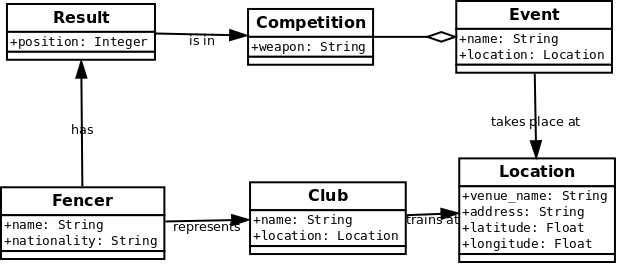
\includegraphics[width=\textwidth]{class_diagram}
    \caption{Class Diagram}
  \end{figure}